\chapter{Résultats et validation}
\label{ch:resultats}

Ce chapitre présente de manière synthétique les résultats obtenus après l’implémentation de la plateforme \textbf{Harmoni}.  
Les captures ci-dessous illustrent l’interface et les principales fonctionnalités validées : modélisation, configuration, exécution, suivi et analyse des processus métier.

\section{Vue générale — Dashboard}

\begin{figure}[H]
    \centering
    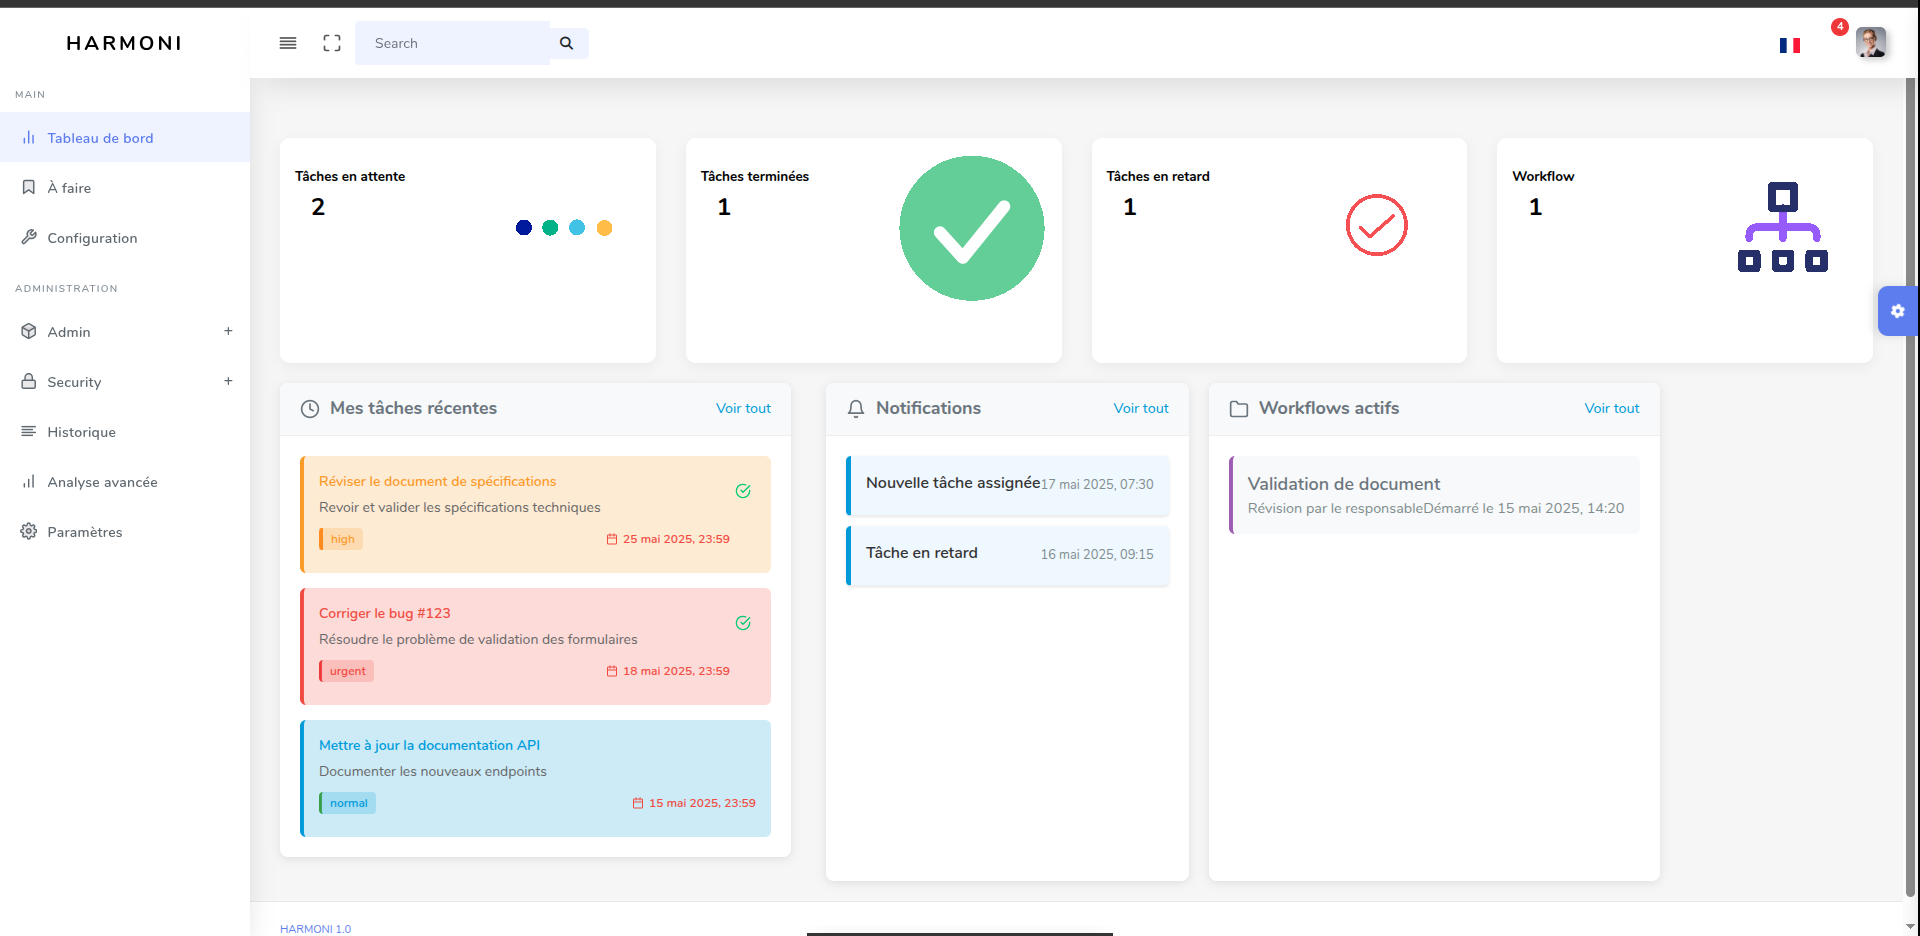
\includegraphics[width=0.9\textwidth]{Images/dashboard.png}
    \caption{Tableau de bord (Dashboard) — vue générale de Harmoni}
    \label{fig:dashboard}
\end{figure}

\paragraph{Description de la capture.}  
La figure~\ref{fig:dashboard} montre le tableau de bord principal : indicateurs-clés (nombre d'instances actives, taux d'échec, temps moyen de traitement), liste d'instances récentes, filtres globaux (par processus, par statut, par utilisateur) et accès rapides aux actions (nouveau modèle, déploiement, rapport). On y voit également des composants graphiques synthétiques (courbes temporelles, gauges).

\paragraph{Interprétation et validation.}  
Ce dashboard illustre la capacité de Harmoni à fournir une supervision centralisée en temps réel. Il valide le besoin de suivi opérationnel (monitoring) et facilite la prise de décision rapide par les gestionnaires de processus. Les KPI démontrent la conformité aux exigences non fonctionnelles en matière d’ergonomie et d’observabilité.

\section{Modélisation BPMN}

\begin{figure}[H]
    \centering
    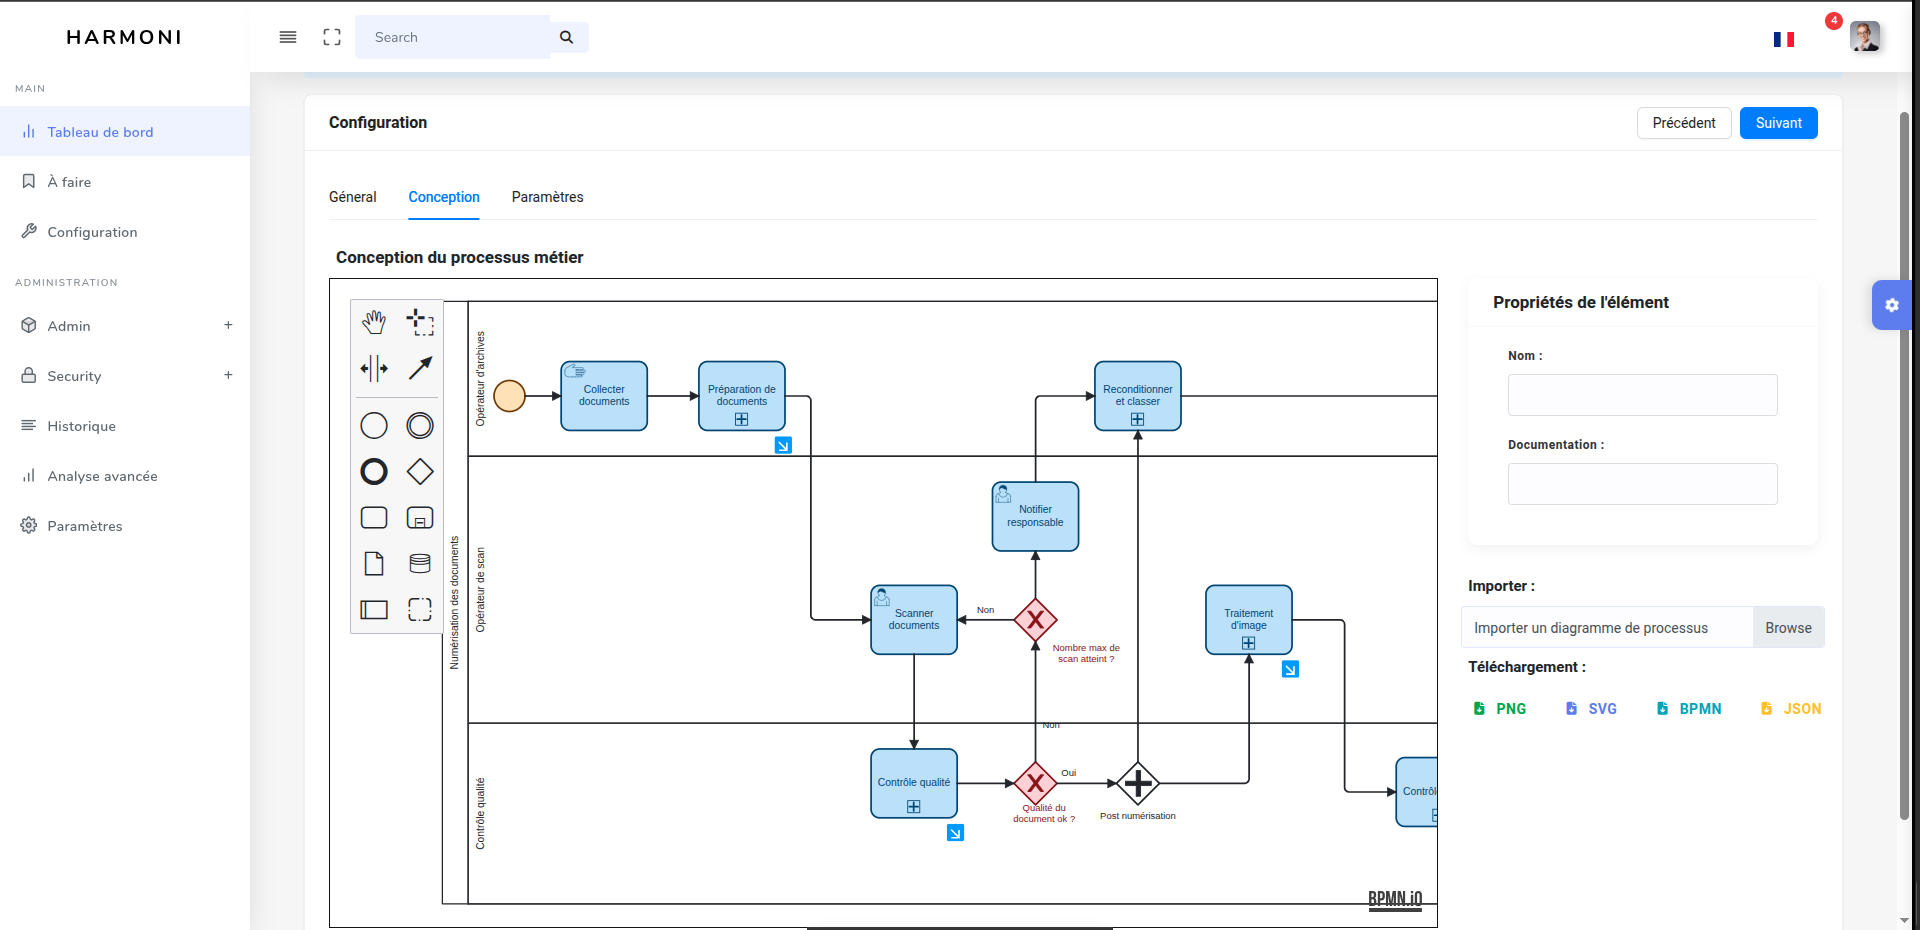
\includegraphics[width=0.9\textwidth]{Images/configuration.png}
    \caption{Éditeur BPMN — modélisation graphique}
    \label{fig:modelisation}
\end{figure}

\paragraph{Description de la capture.}  
La figure~\ref{fig:modelisation} montre l’éditeur intégré (canvas) avec la palette d’éléments BPMN (événements, tâches, passerelles), le panneau de propriétés contextuelles (configuration d’un élément sélectionné) et la barre d’outils (sauvegarde, validation, import/export BPMN XML).

\paragraph{Interprétation et validation.}  
Cette capture confirme que Harmoni permet la création visuelle des processus (glisser-déposer), l’édition des propriétés et la validation syntaxique BPMN. Elle valide le besoin fonctionnel de modélisation intuitive et l’interopérabilité via les formats BPMN standard (import/export).

\section{Configuration des tâches}

\begin{figure}[H]
    \centering
    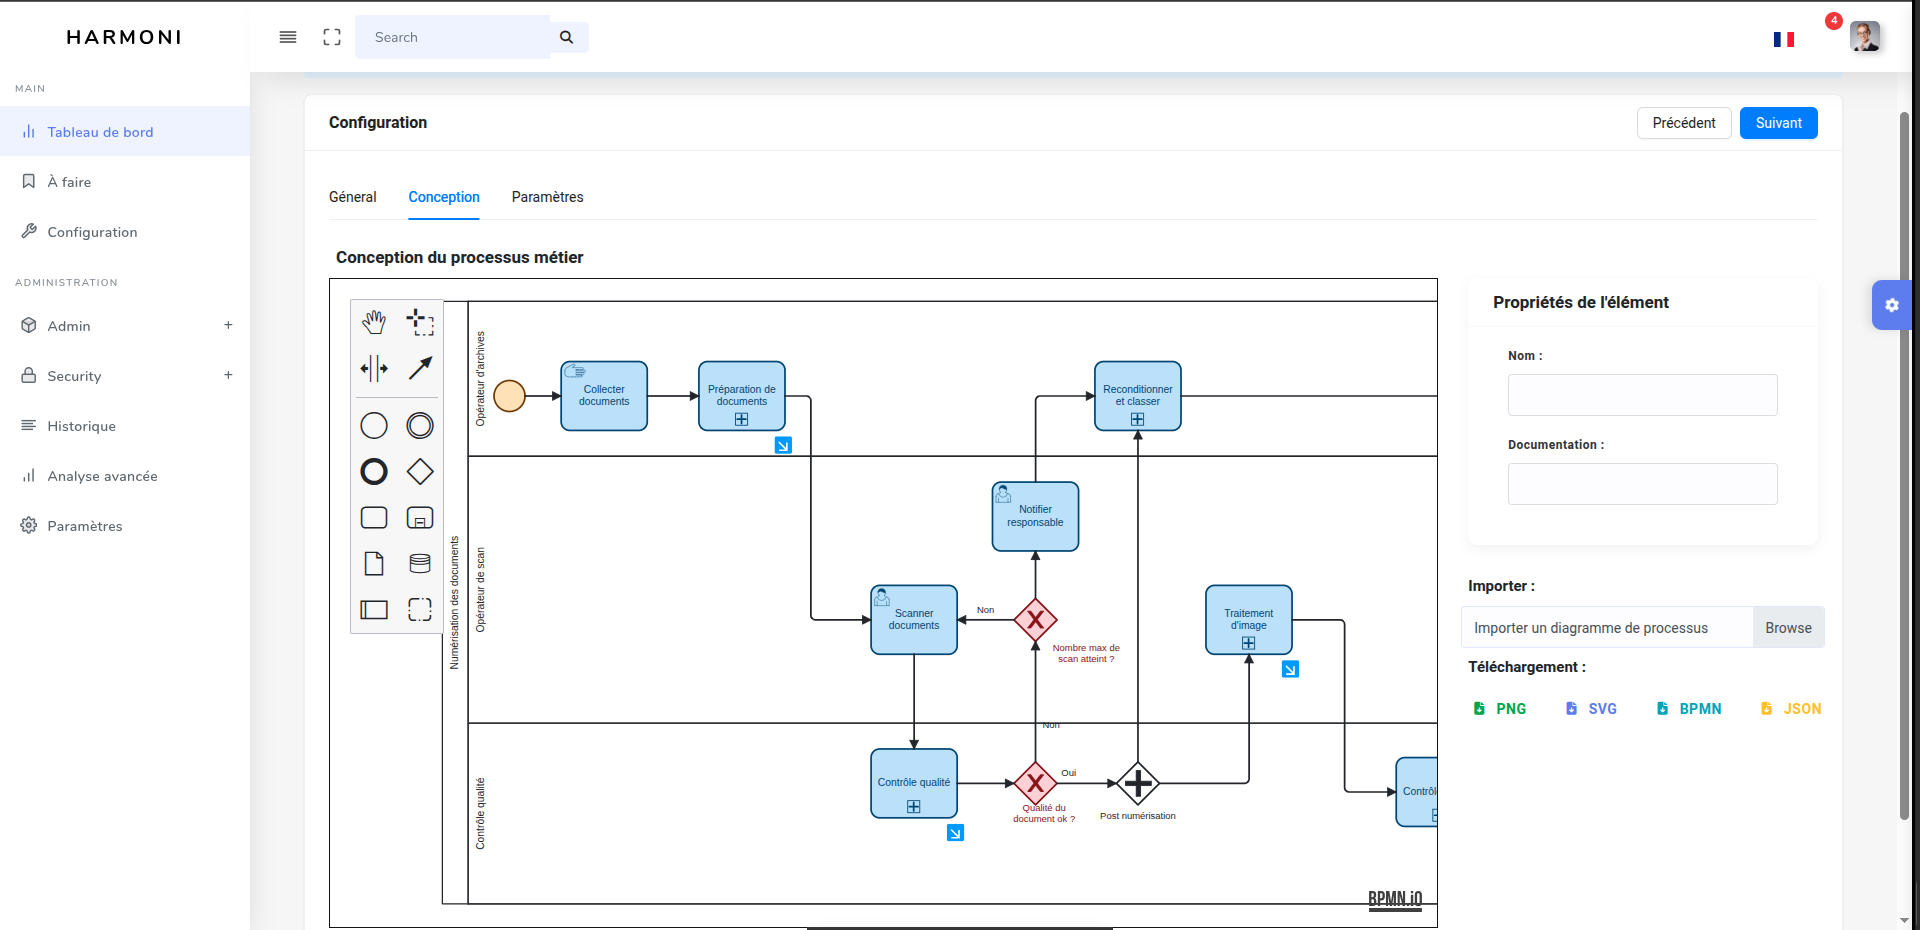
\includegraphics[width=0.9\textwidth]{Images/configuration.png}
    \caption{Configuration d’une tâche — affectation, règles et paramètres}
    \label{fig:configuration}
\end{figure}

\paragraph{Description de la capture.}  
La figure~\ref{fig:configuration} présente le panneau de configuration d’une tâche : affectation par utilisateur/groupe, SLA (délais), paramètres d’exécution (retries, timeout), mappage des variables et hooks de service (appel à un connecteur documentaire).

\paragraph{Interprétation et validation.}  
Cette vue montre comment les décisions de conception (backend Spring Boot + moteur BPMN) sont exposées côté frontend pour permettre une configuration fine des tâches. Elle valide la traçabilité des paramètres d’exécution et la compatibilité avec l’intégration documentaire (connecteurs Kairos).

\section{Kanban utilisateur}

\begin{figure}[H]
    \centering
    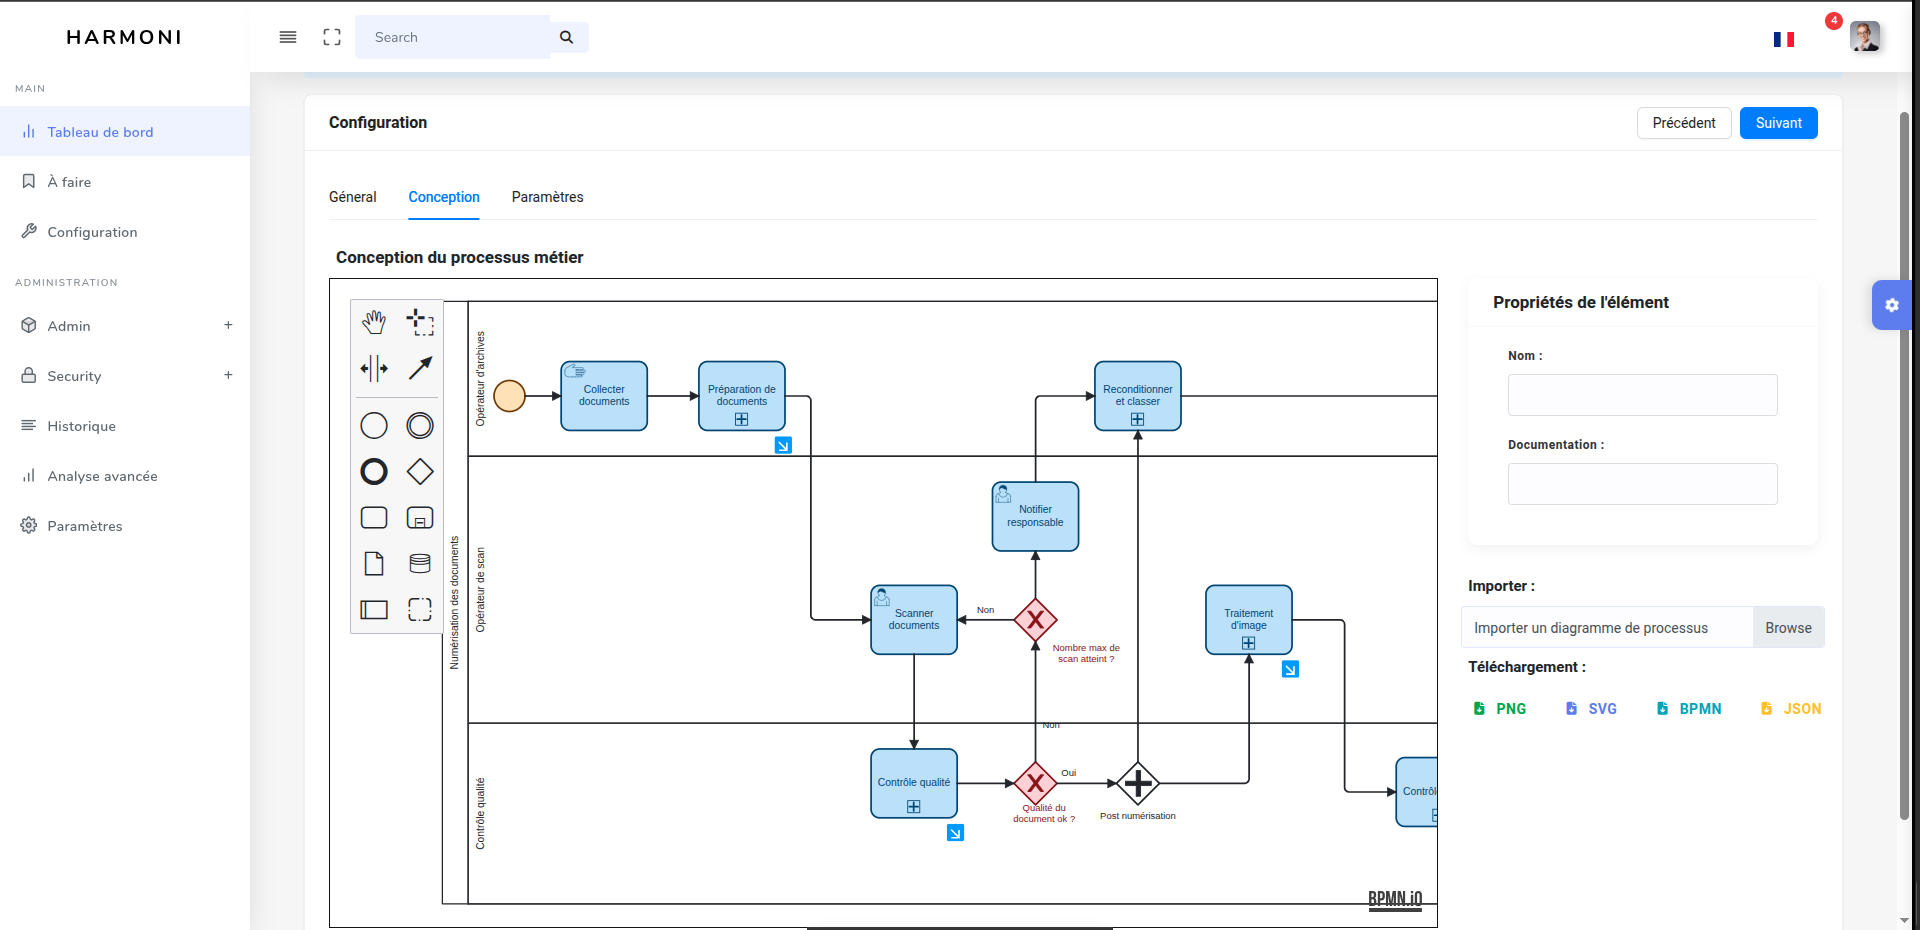
\includegraphics[width=0.9\textwidth]{Images/configuration.png}
    \caption{Tableau Kanban — gestion et priorisation des tâches par utilisateur}
    \label{fig:kanban}
\end{figure}

\paragraph{Description de la capture.}  
La figure~\ref{fig:kanban} illustre le tableau Kanban personnalisé : colonnes par statut (À faire, En cours, En attente, Terminé), cartes représentant les tâches/processus, actions rapides (assigner, commenter, déplacer), filtres et recherche.

\paragraph{Interprétation et validation.}  
Le Kanban traduit la capacité opérationnelle pour les utilisateurs finaux : gestion quotidienne des tâches, priorisation et collaboration. Il valide le besoin fonctionnel d’un tableau de bord utilisateur pratique et montre la synchronisation en temps réel entre le moteur d’exécution et l’interface.

\section{Notifications en temps réel}

\begin{figure}[H]
    \centering
    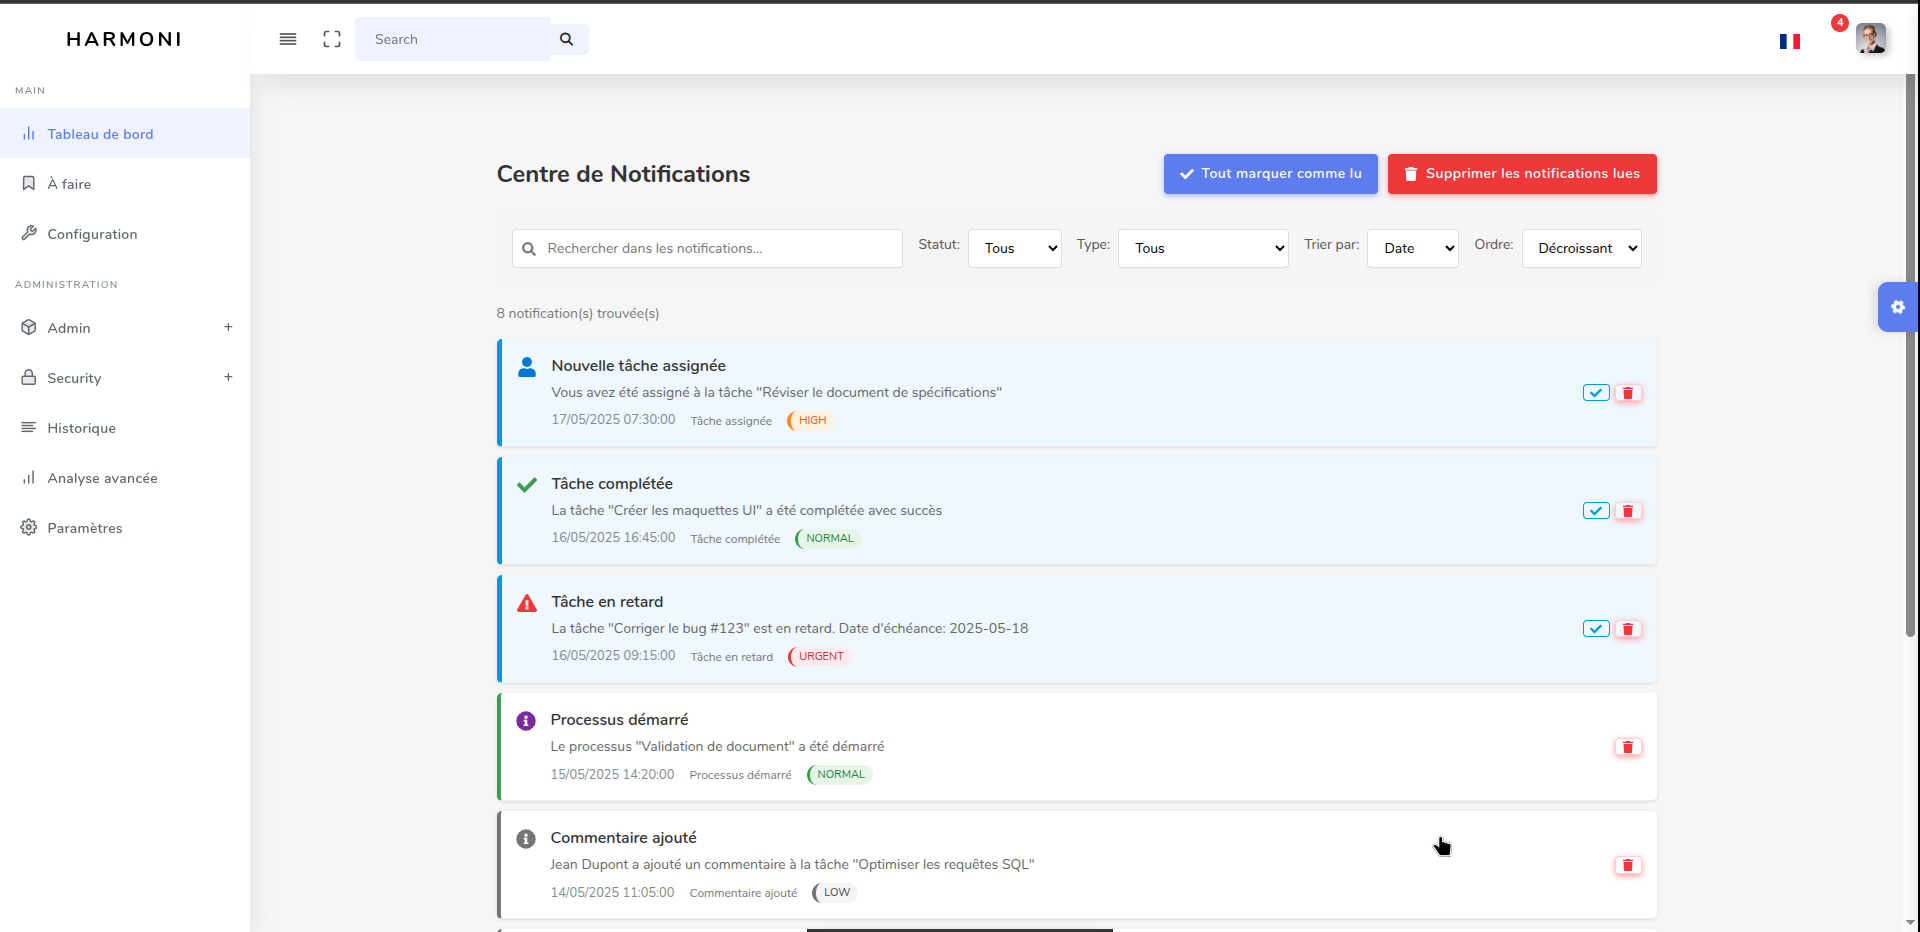
\includegraphics[width=0.9\textwidth]{Images/notification.png}
    \caption{Centre de notifications / alerte en temps réel}
    \label{fig:notification}
\end{figure}

\paragraph{Description de la capture.}  
La figure~\ref{fig:notification} présente l’interface de notifications : toasts en temps réel, historique des notifications, paramétrage des types d’alertes (échec d’instance, dépassement SLA, approbation requise) et liens directs vers l’instance concernée.

\paragraph{Interprétation et validation.}  
Les notifications démontrent la réactivité du système et la capacité à prévenir les acteurs des événements critiques. Elles répondent aux exigences métier d’alerte et de réactivité (SLA) et facilitent l’escalade opérationnelle.

\section{Historique et monitoring}

\begin{figure}[H]
    \centering
    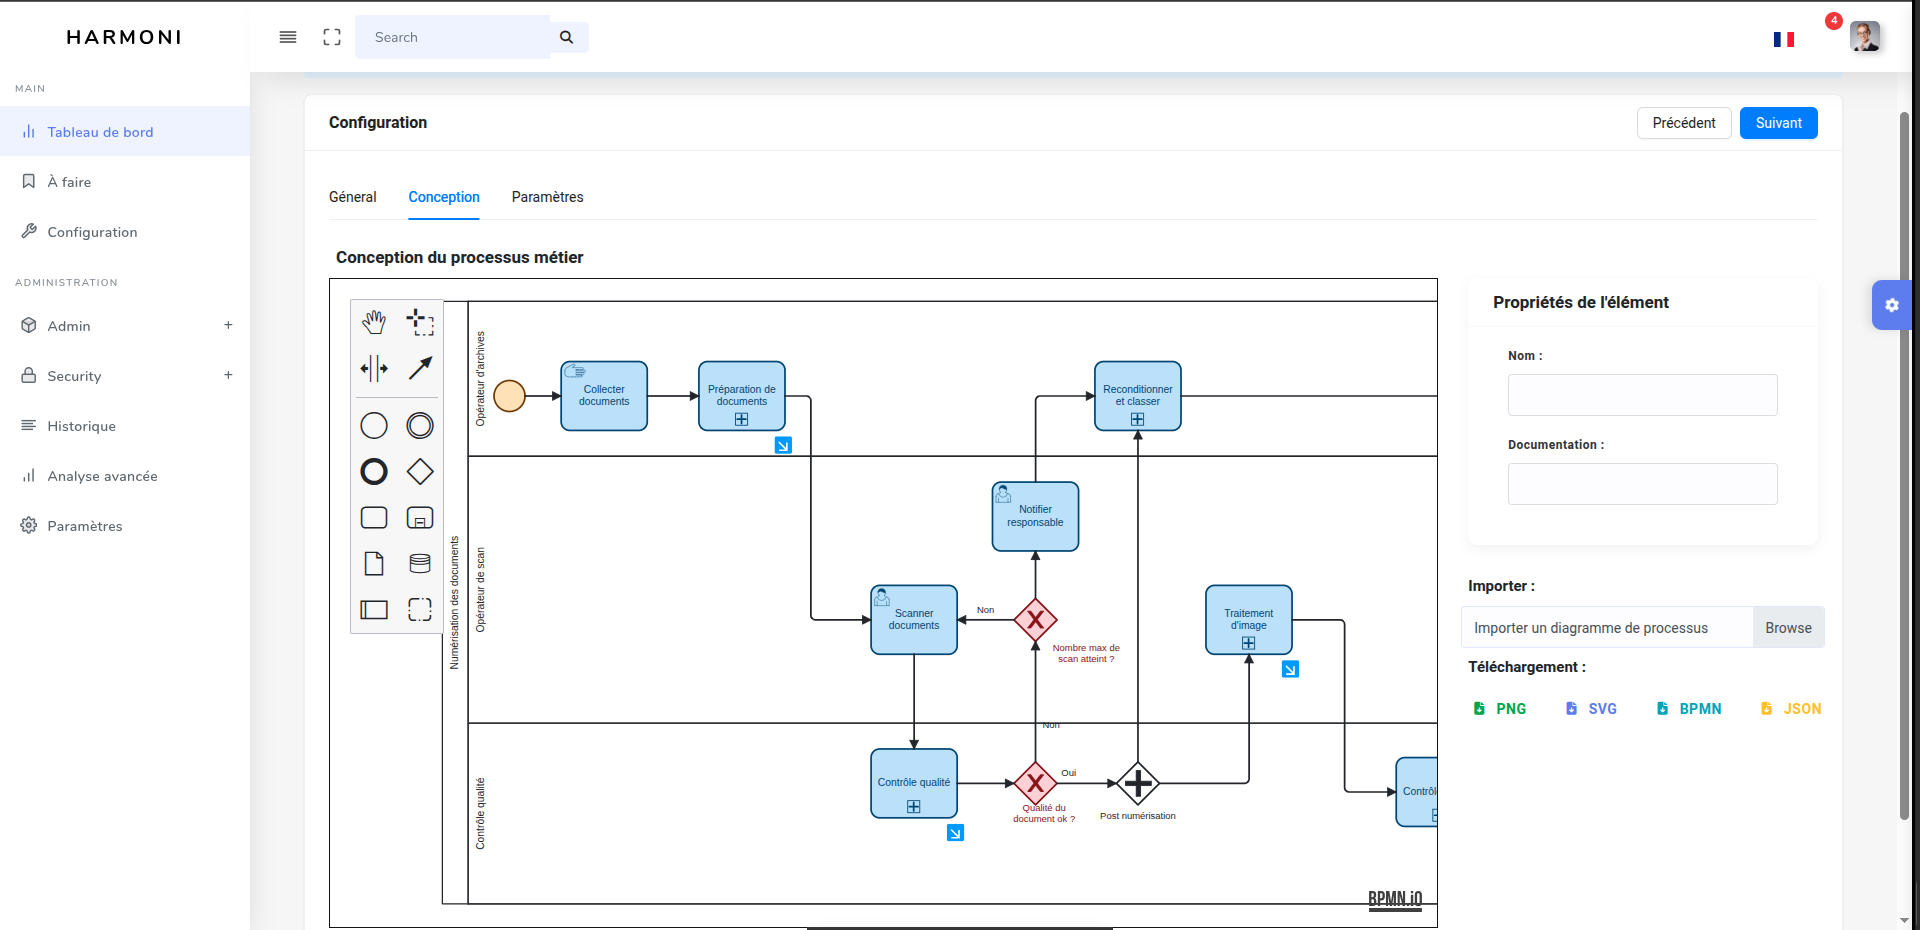
\includegraphics[width=0.9\textwidth]{Images/configuration.png}
    \caption{Historique des exécutions et vue détaillée d’une instance}
    \label{fig:historique}
\end{figure}

\paragraph{Description de la capture.}  
La figure~\ref{fig:historique} montre la liste des instances (actives et terminées), leurs durées, événements marquants, journaux d’exécution et possibilité de relecture / export des logs pour audit.

\paragraph{Interprétation et validation.}  
Cet historique est essentiel pour la conformité et le debugging. Il valide les besoins non fonctionnels liés à la traçabilité, la gouvernance et la fiabilité. Les fonctionnalités d’export et d’archivage facilitent le reporting et les audits internes.

\section{Analyses BPMN avancées}

\begin{figure}[H]
    \centering
    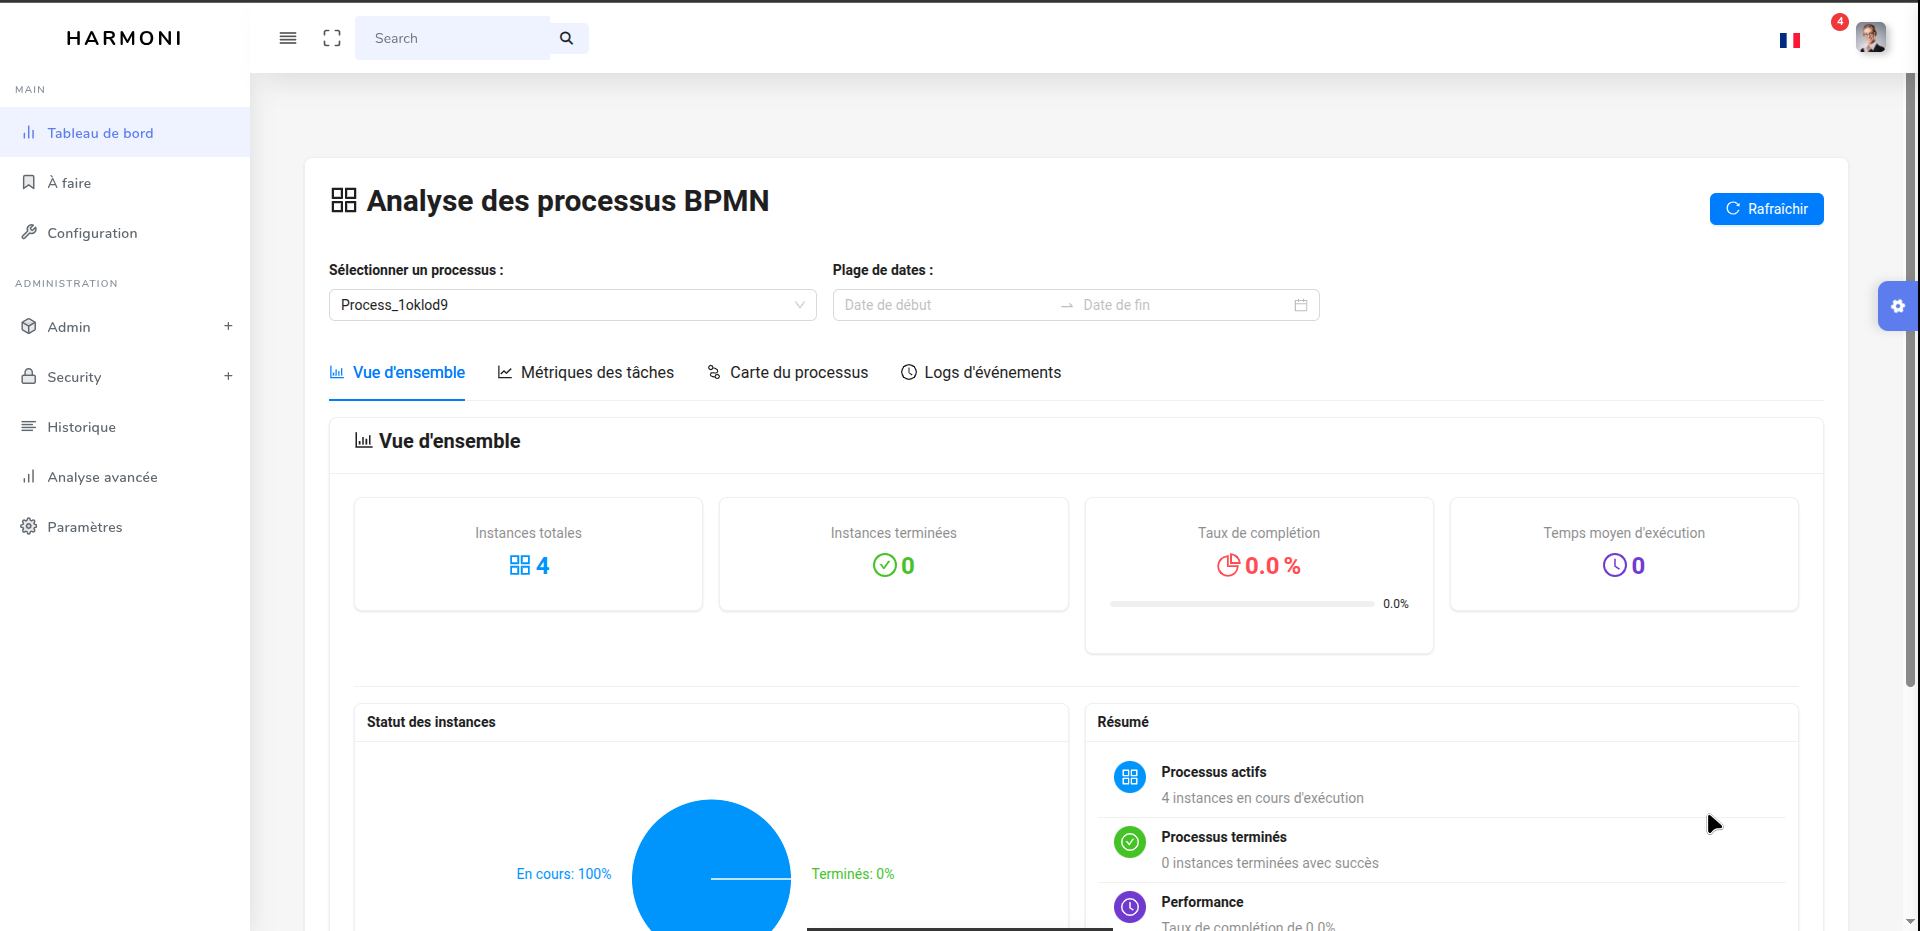
\includegraphics[width=0.9\textwidth]{Images/analyse.png}
    \caption{Module d’analyse — variantes, goulets, prédictions et réseau social organisationnel}
    \label{fig:analyse}
\end{figure}

\paragraph{Description de la capture.}  
La figure~\ref{fig:analyse} illustre l’interface analytique : visualisation des variantes de processus (heatmap / arbres de variantes), histogrammes des temps par activité (goulets d’étranglement), courbes de prédiction de fin d’instance, et graphe de réseau social montrant les interactions entre ressources.

\paragraph{Interprétation et validation.}  
Ces outils analytiques confirment l’apport scientifique et opérationnel de Harmoni :  
\begin{itemize}
    \item \textbf{Analyse des variantes} : identifie les chemins majoritaires et les divergences « as-is » vs modèle théorique ; utile pour prioriser les améliorations.
    \item \textbf{Détection des goulets} : mesure les temps d’attente / traitement et localise les points à optimiser.
    \item \textbf{Prédiction de performance} : fournit des estimations et alertes proactives pour respecter les SLA.
    \item \textbf{Réseau social} : met en évidence les acteurs clés et risques de centralisation des connaissances.
\end{itemize}
Ces outputs valident la valeur ajoutée analytique attendue par Kairos.

\section{Synthèse et recommandations pour les captures}

\paragraph{Synthèse.}  
Les captures présentées démontrent que Harmoni couvre le cycle complet : modéliser, configurer, exécuter, suivre, analyser. Elles valident les exigences fonctionnelles (modélisation, exécution, monitoring) et non fonctionnelles (sécurité, traçabilité, ergonomie).

\paragraph{Recommandations pour finaliser les images (à insérer) :}
\begin{itemize}
    \item Annoter chaque capture avec des encadrés ou flèches pour pointer les éléments importants (KPI, boutons d’action, zones de configuration).
    \item Pour le dashboard, indiquer les valeurs numériques clés (ex. : nombre d’instances actives, temps moyen).
    \item Pour l’éditeur BPMN, afficher une validation d’erreur ou réussite pour démontrer la vérification syntaxique.
    \item Pour l’analyse, ajouter une courte légende expliquant comment lire la heatmap / graphe.
    \item Prévoir une capture montrant un flux de notification -> action (ex. : notification qui mène à la fiche d’instance).
\end{itemize}

\bigskip
Ces descriptions intégrées à chaque capture rendent le chapitre plus lisible et démontrent précisément comment chaque écran répond à un besoin du projet.
